\section{Contribuindo com plataformas abertas} % (fold)
\label{sec:contribuindo_com_plataformas_abertas}

Um dos intuitos deste trabalho baseia-se em contribuir com uma aplicação \textit{open-souce} disponível na plataforma \href{GitHub.com}{GitHub}. A seguinte sessão se destina em apresentar a forma como tais contribuições podem ser realizadas. Devido ao repositório do APT esta armazenado no GitHub, a sessão pode se tornar tendenciosa, porém o conceito de \textit{pull-request} ou  \textit{merge-request} requeste é amplamente utilizado em outras plataformas de contribuição, como \href{https://bitbucket.org/}{Bitbucket}, \href{https://gitlab.com/}{GitLab} ou ate mesmo \href{http://sourceforge.net/}{SourceGorge}


\subsection*{Mantendo uma copia} % (fold)
\label{sub:mantendo_uma_copia_sua}


Normalmente não temos autorização pra alterar as informações de outra pessoa sem seu consentimento. Da mesma forma  é com os repositórios {\code git}. Assim, um dos primeiros passos para começar a contribuir com uma ferramenta \textit{open-source} é fazer uma copia dela em seu repositório. Essa cópia pode ser feita de duas formas basicamente, no intuito de manter os autores das modificações anteriores:

\begin{description}
	\item [\textit{Fork}]: O termo é amplamente utilizado quando queremos fazer uma copia de um repositório para a nossa conta em uma mesma plataforma. Normalmente este passo é realizado via interface gráfica, ainda no navegador. Na \cref{fig:github_fork} é possível observar o botão no canto superior direito indicado para realizar um \textit{fork} do atual repositório.

	\begin{figure}[h]
	  \centering
		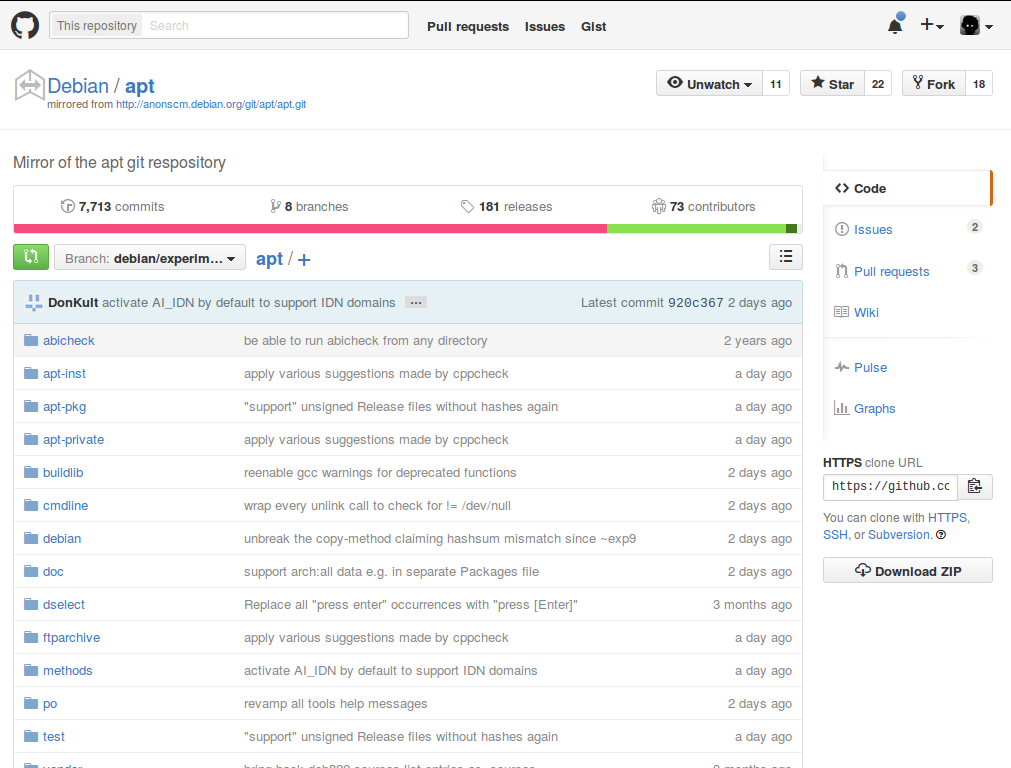
\includegraphics[width=0.85\textwidth]{figuras/fork}
	  \caption{Visão de um repositório do \textit{GitHub}}
	  \label{fig:github_fork}
	\end{figure}

	\item [\textit{Adicionando \textit{remote}}]: Quando desejamos realizar uma copia do repositório em uma plataforma distinta da original, a forma mais simples de proceder é clonando o repositório e incluindo nele um novo \textit{remote} para a nova plataforma. Assim conseguimos trabalhar com a mesma arvore de \textit{commits} do repositório original, mantendo os créditos e alterações originais.
\end{description}
% subsection mantendo_uma_copia_sua (end)

\subsection*{Evoluindo o código} % (fold)
\label{sub:evoluindo_o_c_digo}

Nesto ponto de contribuição, o contribuinte desenvolve o código semelhante ao processo de produção de código pessoal. O código já esta em um repositório pessoal e o usuário já possui todos os direitos administrativos do repositório. Obviamente que caso a contribuição esteja sendo feita à uma aplicação grande e com muitos contribuidores, é importante se manter sincronizado com o código original, para evitar que o retorno da contribuição não seja tão trabalhoso para o revisor, além de evitar situações de confitos.
% subsection evoluindo_o_c_digo (end)

\subsection*{Retornando sua contribuição} % (fold)
\label{sub:retornando_sua_contribui_o}

Quando se decidido que a contribuição já esta a um ponto aceitável para encaminha-la de volta para o código original, é o momento de se realizar o \textit{pull-request}\footnote{Ou \textit{merge-request} dependendo do ambiente de desenvolvimento em que esteja-se contribuindo.}. Uma contribuição é interessante quando possui as seguintes características:


\begin{itemize}
	\item Evolução de código mantendo os padrões de guia de estilo definido pelo desenvolvedor original/linguagem.
	\item Testes para a evolução de código proposto.
	\item Documentação da feature implementada ou atualização da documentação como reflexão das modificações sugeridas.
\end{itemize}
% subsection retornando_sua_contribui_o (end)

Realizada a contribuição, é dever do mantenedor do repositório original revisar o código e decidir se deve ou não aceita-lo.

% section contribuindo_com_plataformas_abertas (end)


\section{Primeira contribuição} % (fold)
\label{sec:primeira_contribui_o}

A primeira contribuição tinha como objetivos a ambientalização com o ambiente e o time oficial de desenvolvimento. Como tarefa, foi definido a implementação minima de uma estrutura que permita um contexto de ordenação que possa ser definido pelo usuário. O intuito era oferecer as seguintes opções de ordenação na primeira contribuição:

\begin{description}
	\item [\textit{Alphabetic}] Ordenação padrão em ordem alfabética. Os pacotes são ordenados de acordo com seu nome.
	\item [\textit{Reverse Alphabetic}] Semelhante a ordenação alfabética, porém em ordem decrescente, ou seja, palavras que começam com {\code Z} são apresentadas antes das iniciadas com {\code A}.
	\item [\textit{Status}] Ordena os pacotes de acordo com as seguintes características:
	\begin{enumerate}
		\item Desinstalado,
		\item Instalado e com possível atualização,
		\item Instalado via pacote local,
		\item Instalado e descartável (auto removível),
		\item Instalado automaticamente,
		\item Instalado,
		\item Atualizável,
		\item om configuração residual
	\end{enumerate}
	\item [\textit{Version}] Ordena a saída de acordo com a versão da aplicação.
\end{description}

\subsection*{Alteração da estrutuda de dados} % (fold)
\label{sub:altera_o_da_estrutuda_de_dados}

Originalmente, os dados eram armazenados em um {\code map}, visto que essa estrutura não permite a duplicação de chaves e possui uma ordenação alfabética automática. Todavia, alterar o algoritmo de ordenação de um {\code map} ocorrem em seu tempo de declaração. Esta condição inviabiliza a possibilidade de alterar a ordenação através de uma \textit{flag} como parâmetro de execução. Visto essa condição, a estrutura foi atualizada para a estrutura de dados {\code vector}.

A inserção de candidatos na saída do APT ocorre de acordo com os repositórios inseridos no {\code source.list} da distribuição. Isso implica que apenas adicionar candidatos no vetor implicaria em uma ordenação com baixa precisão, visto que a sequência de repositórios variaria de usuário para usuário. Assim, a simples troca de estrutura de dados de {\code map} para {\code vector} implica na necessidade de implementar o método de ordenação alfabética, antes nativamente implementado pela estrutura {\code map}.
% subsection altera_o_da_estrutuda_de_dados (end)

% section primeira_contribui_o (end)